\documentclass[12pt]{article}
\usepackage{amsmath}
\usepackage{tikz}
\usepackage[simplified]{pgf-umlcd}
\usepackage{parskip}
\usepackage{verbments}

\usepackage[letterpaper]{geometry}
\geometry{left=.5in, right=.5in}



\newcommand{\classname}[1]{\texttt{#1}}


\title {OpenMDAO 1.0 Design Doc}

\begin{document}
\maketitle

\section{Analysis Composition Objects}

OpenMDAO is designed around the Multidisciplinary Analysis and Unfied Derivatives (MAUD) mathematical
architecture. In MAUD, all analyses are represented as systems of coupled non-linear implicit equations.
\classname{System} is the baseclass for all objects that are responsible for mathematical computations.
Any instance of \classname{System} must implement 5 methods in order to be able to perform
analysis:

\begin{itemize}
    \item apply\_nonlinear: solve for the residual values given the values for
    the inputs and states
    \item solve\_nonlienar: given values for the inputs, find the values of the
    state variables that drive the non linear residual equations to zero
    \item linearize: compute partial derivatives around current location for all
    residuals as a function of current input and state variables
    \item apply\_linear: linear operator which provides the product of the systems
    Jacobian with a given vector
    \item solve\_linear: solve the linear system defined by the jacobian on the
    lhs and a given vector on the right hand side
\end{itemize}



The basic unit of computational work in OpenMDAO is the \classname{Component}.
The apply\_linear method in \classname{System} is intended to take advantage of sparse jacobian
structures and provide an efficient method of performing matrix vector products. In some cases,
such as when wrapping a CFD code, this method will be ultimately performed by an underlying
linear operator in the analysis tool. However, for many cases when analyses are developed natively in
OpenMDAO, the user may find it convinent to provide a Jacobian in the form of a dictionary with
keys of $(<output\_var>,\ <input\_var>)$ and values being partial derivatives of
$\frac{d<output\_var>}{d<input\_var>}$. This dictionary is given as the return value
from the linearize method. The base implementation of the apply\_linear method
in \classname{ImplicitComponent} will automatically implement the linear operator around
the given dictionary. The user is expected to overload the base class method if they wish to
use implement the linear operator themselves.

\begin{center}
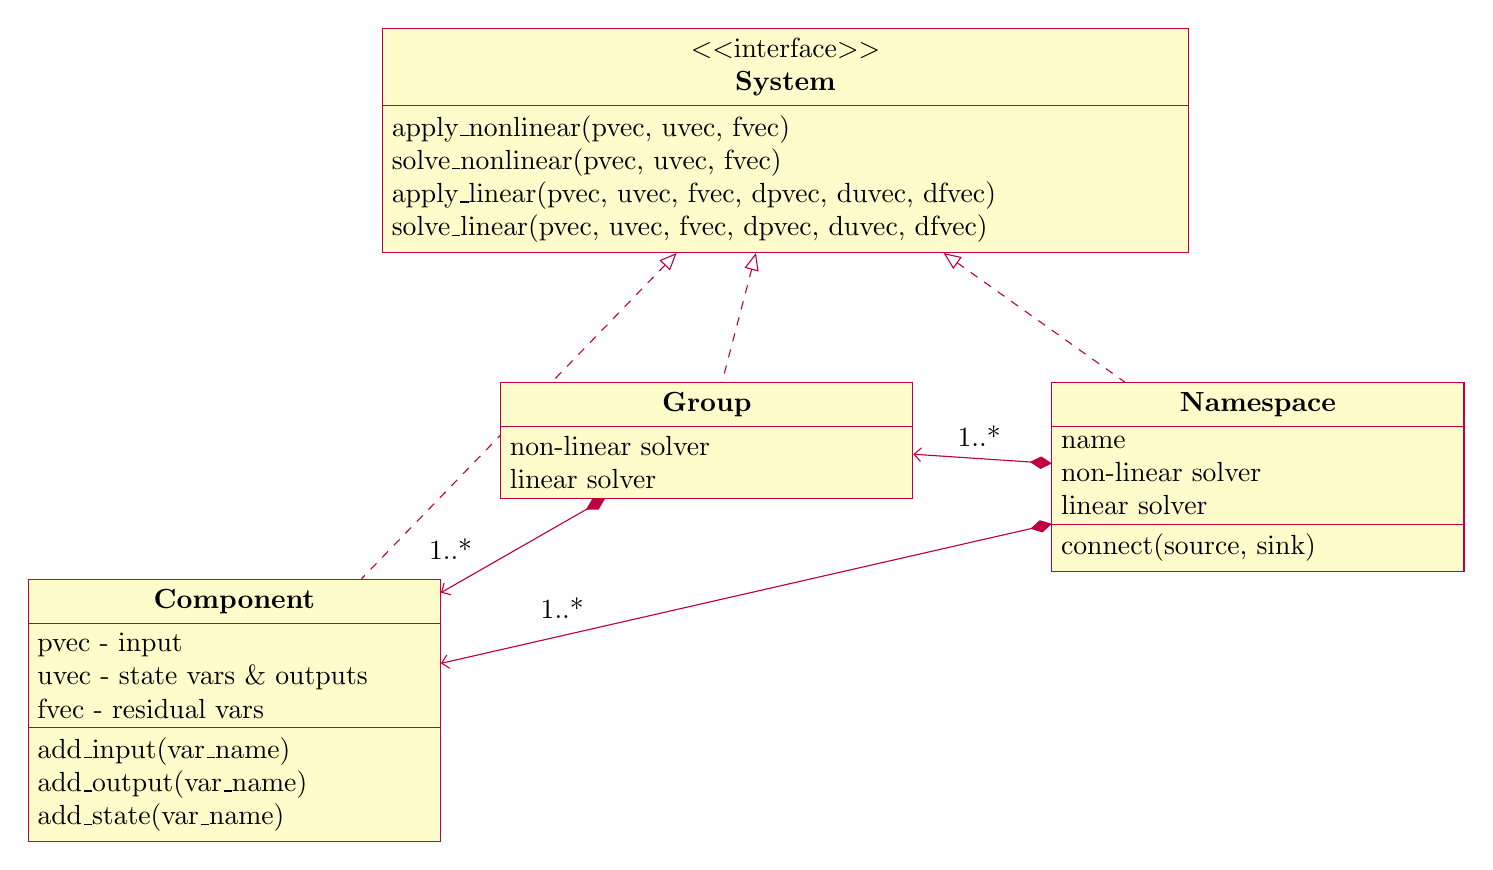
\begin{tikzpicture}[]% [ show background grid ]
    \begin{interface}[text width =10cm ]{System}{0,0}
        \operation{apply\_nonlinear(pvec, uvec, fvec)}
        \operation{solve\_nonlinear(pvec, uvec, fvec)}
        \operation{apply\_linear(pvec, uvec, fvec, dpvec, duvec, dfvec)}
        \operation{solve\_linear(pvec, uvec, fvec, dpvec, duvec, dfvec)}
    \end{interface}

    \begin{class}{Component}{-7,-7}
        \implement{System}
        \attribute{pvec - input}
        \attribute{uvec - state vars \& outputs}
        \attribute{fvec - residual vars}
        \operation{add\_input(var\_name)}
        \operation{add\_output(var\_name)}
        \operation{add\_state(var\_name)}

    \end{class}

    \begin{class}{Group}{-1,-4.5}
        \implement{System}
        \attribute{non-linear solver}
        \attribute{linear solver}
    \end{class}

    \begin{class}{Namespace}{6,-4.5}
        \implement{System}
        \attribute{name}
        \attribute{non-linear solver}
        \attribute{linear solver}
        \operation{connect(source, sink)}
    \end{class}

    \composition{Group}{}{1..*}{Component}
    \composition{Namespace}{}{1..*}{Component}
    \composition{Namespace}{}{1..*}{Group}

\end{tikzpicture}
\end{center}

\pagebreak
\section{Defining Component Classes}

Componnets can have implicit and explicit relationships. Implicit replationships are defined
by adding state variables. Explicit relationships are defined by adding outputs.


\begin{pyglist}[language=python]
    class SomeComp(Component):
        def __init__(self):
            super(SomeComp,self).__init__()

            self.add_input('x1', size=(2,3))
            self.add_input('x2', val=3.4)

            self.add_state('y1', size=(2,3))
            self.add_output('z1', size=(2,3))

        def apply_nonlinear(self, pvec, uvec, fvec):

            uvec['z1'] = 3*pvec['x1'] + pvec['x2']
            fvec['y1'] = uvec['y1'] - pvec['x1']

        def linearize(self):
            pass # nothing meaningful to do here

        def apply_linear(self, pvec, uvec, dpvec, duvec, dfvec, mode='fwd'):

            if mode="fwd":
                duvec['z1'] += 3*dpvec['x1']
                duvec['z1'] += dpvec['x2']
                dfvec['y1'] += duvec['y1'] - dpvec['x1']

            elif mode='adj':
                dpvec['x1'] += 3*duvec['z1']
                dpvec['x2'] += duvec['z1']

                duvec['y1'] += dfvec['y1']
                dpvec['x1'] -= dfvec['y1']
\end{pyglist}

Users building a component can choose to return a dictionary from linearize to avoid
writing apply\_linear method themselves.

\begin{pyglist}[language=python]
    class SomeOtherComp(Component):
        def __init__(self):
            super(SomeComp,self).__init__()

            self.add_input('x1', size=(2,3))
            self.add_input('x2', val=3.4)

            self.add_state('y1', size=(2,3))
            self.add_output('z1', size=(2,3))

        def apply_nonlinear(self, pvec, uvec, fvec):

            uvec['z1'] = 3*pvec['x1'] + pvec['x2']
            fvec['y1'] = uvec['y1'] - pvec['x1']

        def linearize(self):
            self.J = {}
            self.J['z1','x1'] = 3
            self.J['z1','x2'] = 1

            self.J['y1'] = 1 # derivative of resid w.r.t state
            self.J['y1','x1'] = -1

            return J
\end{pyglist}

Another part of the component api, \textttt{multi_apply_linear}, allows a component
to provide matrix vector products with multiple right-hand-sides at once.

\begin{pyglist}[language=python]
    class SomeComp(Component):
        def __init__(self):
            super(SomeComp,self).__init__()

            self.add_input('x1', size=(2,3))
            self.add_input('x2', val=3.4)

            self.add_state('y1', size=(2,3))
            self.add_output('z1', size=(2,3))

        def apply_nonlinear(self, pvec, uvec, fvec):

            uvec['z1'] = 3*pvec['x1']**2 + pvec['x2']
            fvec['y1'] = uvec['y1'] - pvec['x1']

        def linearize(self):
            pass # nothing meaningful to do here

        def multi_apply_linear(self, pvec, uvec, dpmat, dumat, dfmat, mode='fwd'):

            if mode="fwd":
                dumat['z1'] += 3*2*pvec['x1'].dot(dpmat['x1'])
                dumat['z1'] += dpmat['x2']
                dfmat['y1'] += dumat['y1'] - dpmat['x1']

            elif mode='adj':
                dpmat['x1'] += 3*2*pvec['x1'].dot(dumat['z1'])
                dpmat['x2'] += dumat['z1']

                dumat['y1'] += dfmat['y1']
                dpmat['x1'] -= dfmat['y1']
\end{pyglist}

default base-class implementation that is just a for-loop over apply\_linear.

\section{Variable Connections within a namespace}
\subsection{Auto Connect (Global Variables)}
\subsection{Manual Connection (Local Variables)}

\section{Drivers  (Optimizers and DOE)}
Note: Linear and non-linear solvers do not count as drivers

Drivers are iterative processes that operate on top of analyses


\end{document}
